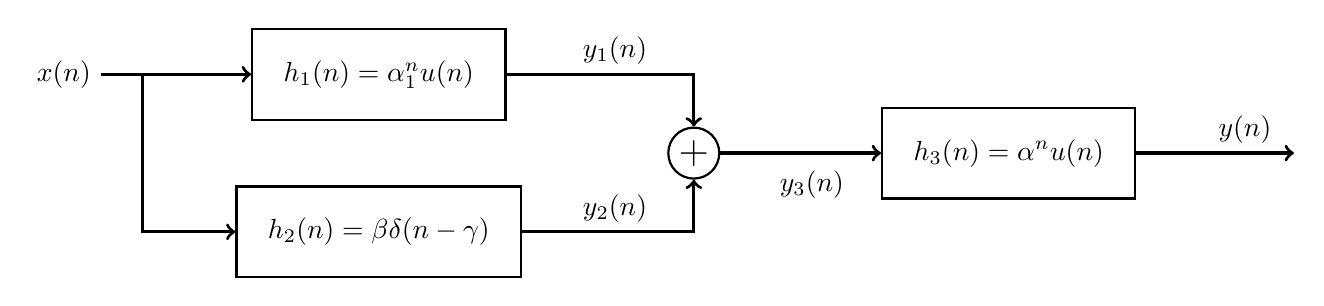
\begin{tikzpicture}
    \node[circle,draw,thick,inner sep=0.05cm] (plus) at (0,0) {\Large +} ;
    \node[rectangle,draw,thick,inner sep=0.4cm] (h1) at (-4,1) {$h_1(n)=\alpha_1^n u(n)$} ;
    \node[rectangle,draw,thick,inner sep=0.4cm] (h2) at (-4,-1) {$h_2(n)=\beta \delta(n-\gamma)$} ;
    \node[rectangle,draw,thick,inner sep=0.4cm] (h3) at (4,0) {$h_3(n)=\alpha^n u(n)$} ;
    \node[xshift=-4cm] (x_n) at (h1) {$x(n)$} ;
    \node[xshift=-3cm,inner sep=-0.1] (x_n_arrow_cross) at (h1) {} ;

    \node[xshift=3cm,yshift=.3cm] (y_1) at (h1) {$y_1(n)$} ;
    \node[xshift=3cm,yshift=.3cm] (y_2) at (h2) {$y_2(n)$} ;
    \node[xshift=-2.5cm,yshift=-.4cm] (y_3) at (h3) {$y_3(n)$} ;
    \node[xshift=3cm,yshift=.3cm] (y_n) at (h3) {$y(n)$} ;

    \draw[->, very thick] (x_n) -- (h1.west) ;
    \draw[->, very thick] (x_n_arrow_cross) |- (h2.west) ;
    \draw[->, very thick] (h1.east) -| (plus.north) ;
    \draw[->, very thick] (h2.east) -| (plus.south) ;
    \draw[->, very thick] (plus.east) -- (h3.west) ;
    \draw[->, very thick] (h3.east) -- ++(2,0) ;
\end{tikzpicture}